\documentclass[10pt,twocolumn]{article}
\usepackage{times}
\usepackage[a4paper,margin=1in]{geometry}
\usepackage{url}
\usepackage{hyperref}
\usepackage{float}
\usepackage{amsmath}
\usepackage{amsfonts}
\usepackage{algorithm}
\usepackage{algpseudocode}
\usepackage{booktabs}
\usepackage{multirow}
\usepackage{graphicx}
\usepackage{placeins}

\hbadness=9999
\hfuzz=2pt
\hyphenpenalty=10000
\exhyphenpenalty=10000
\sloppy

\title{\textbf{Elevator Dispatching using Reinforcement Learning}}
\author{
\textbf{Devadatta Mahesh Pokharanakar (142502012)}
}
\date{\today}

\begin{document}
\twocolumn[
\maketitle
]

\section*{Abstract}
This project explores the application of Reinforcement Learning (RL) to optimize elevator dispatching in multi-floor, multi-elevator buildings. Traditional rule-based elevator control systems often struggle to adapt to dynamic traffic patterns and optimize multiple objectives simultaneously. I developed a comprehensive simulation environment modeling realistic elevator physics, and various traffic patterns. I implemented multiple RL algorithms including PPO, A2C, DQN, SAC, TD3, DDPG, and their variants and evaluated them against traditional rule-based systems. The system incorporates enhanced state representations, diverse reward functions, and specialized action spaces inspired by recent research. Performance was assessed using metrics such as average waiting time, passenger throughput, elevator utilization, and fairness. While RL agents achieved comparable performance to rule-based systems, challenges in energy efficiency were identified, suggesting the need for hybrid approaches combining learning with domain constraints.

\section{Objectives}
\begin{enumerate}
    \item Create a detailed elevator simulation with realistic physics, door operations, and passenger behavior patterns.
    \item Train and compare various RL agents including value-based, policy-based, and actor-critic methods.
    \item Develop enhanced observation spaces incorporating elevator states, passenger information, and traffic patterns.
    \item Design and test multiple reward structures balancing efficiency, fairness, and energy considerations.
    \item Establish comprehensive evaluation metrics including passenger waiting times, throughput, and system efficiency.
    \item Benchmark RL performance against conventional rule-based elevator control systems.
\end{enumerate}

\section{Motivation}
Reinforcement learning (RL) offers a principled framework for learning control policies through interaction with the environment, making it a strong candidate for problems involving uncertainty, sequential decisions, and long-term rewards. Historically, RL has been successfully applied to several influential benchmark problems, including Samuel’s checkers player, TD-Gammon, the Acrobot, dynamic channel allocation, and job-shop scheduling---with \emph{elevator dispatching} explicitly recognized as one of the canonical industrial case studies. 

Elevator control is described as:
\begin{quote}
\emph{``A good example of a stochastic optimal control problem of economic importance that is too large to solve by classical techniques such as dynamic programming. Waiting for an elevator is a situation familiar to all of us. How long we wait depends on the dispatching strategy: if passengers on several floors request pickups, which should be served first, and how should elevators position themselves when idle?''}~\cite{MARK2005}
\end{quote}

Elevator dispatching represents a complex sequential decision-making problem under uncertainty. Traditional control systems rely heavily on handcrafted heuristic rules that, while efficient in predictable conditions, lack the adaptability required to handle varying traffic patterns, changing passenger behavior, and multi-objective optimization needs. The elevator group control problem (EGCP) is characterized by:
\begin{enumerate}
    \item \textbf{High-dimensional state space:} Multiple elevators, diverse floor configurations, and stochastic passenger arrivals
    \item \textbf{Dynamic environment:} Strong temporal variation in traffic intensity (up-peak, down-peak, lunchtime, mixed)
    \item \textbf{Multiple competing objectives:} Minimizing waiting time, journey time, and energy consumption while maintaining fairness
    \item \textbf{Real-time decision making:} Policies must react within milliseconds to new hall calls and car events
\end{enumerate}

Despite its presence in RL literature for decades, large-scale deployment of RL-based elevator control has been limited. Existing work often focuses on simplified environments, restricted action spaces, or handcrafted reward functions, leaving several open questions:
\begin{itemize}
    \item Why are modern RL methods (PPO, SAC, TD3, DQN variants) not yet widely adopted in real elevator systems?
    \item Do contemporary algorithms actually outperform well-tuned rule-based dispatchers under realistic conditions?
    \item What practical limitations---energy usage, fairness, stability, training complexity---prevent real-world deployment?
\end{itemize}

These gaps formed the motivation for this work. After reviewing the literature, I became particularly interested in understanding whether modern RL algorithms could meaningfully improve elevator dispatching and what challenges would arise in practice. Moreover, despite the long-standing interest in elevator control as an RL benchmark, I found no publicly available, complete, or actively maintained implementations of modern RL approaches for this problem. This lack of accessible code further motivated the development of a fully reproducible simulation and training framework, systematic evaluation of multiple RL families, and analysis of their strengths, limitations, and deployment feasibility as part of this work.

\section{State-of-the-Art}

\subsection{Algorithmic Approaches}

Early work by Crites and Barto  pioneered a multi-agent Q-learning framework in which each elevator operates as an independent Q-learning agent, with neural networks used to approximate value functions\cite{CRITES1995}. Later research by Yuan et al.\ adopted both model-based (Q-value iteration) and model-free (Q-learning) strategies with discrete state spaces and Boltzmann exploration\cite{YUAN2008}.

More recent systems increasingly rely on deep RL. Vaartjes et al.\ introduced a Dueling Double Deep Q-Network (D3QN) with advanced action-space structures, comparing combinatorial and branching action formulations\cite{VAARTJES2025}. Wan et al.\ further extended D3QN techniques within a Semi-Markov Decision Process (SMDP) framework to better capture the continuous-time nature of elevator dynamics, incorporating temporal grouping and gradient surgery to stabilize training across diverse traffic patterns\cite{WAN2024}.

Although not purely RL, several hybrid approaches exist. For instance, Sorsa et al.\ employed a genetic algorithm for upper-level hall call assignment while using certainty-equivalent control for car-level routing\cite{SORSA2009}. These hybrid frameworks illustrate the value of combining stochastic optimization with RL-style decision-making.

A consolidated comparison of RL algorithms used in elevator dispatching is provided in Appendix Table~\ref{tab:rl-algorithms}.

\subsection{State Representations}

State formulation is a central design choice for elevator dispatching systems. Across the literature, common state variables include:

\begin{itemize}
    \item \textbf{Hall call information}: binary indicators of pending up/down calls per floor, along with elapsed waiting time for each call.
    \item \textbf{Elevator status}: current floor (absolute or normalized), movement direction, velocity, current load level, and lists of allocated destination floors.
    \item \textbf{System-level features}: time of day, traffic intensity indicators, and the relative positions of other elevators.
\end{itemize}

Modern systems extend these features considerably. Vaartjes et al.\ incorporated Estimated Time to Destination (ETD) scores, elevator busyness measures, and fine-grained temporal descriptors (e.g.\ day of week)\cite{VAARTJES2025}. Wan et al.\ augmented the state with passenger arrival rate estimates derived from both historical and real-time data, enabling the agent to explicitly condition its behaviour on dynamic traffic patterns\cite{WAN2024}.
Typical and advanced state features used across the literature are summarized in Appendix Table~\ref{tab:state-repr}.

\subsection{Action Spaces}

RL formulations differ significantly in their treatment of the action space. Two broad classes are observed:

\begin{itemize}
    \item \textbf{Per-elevator control}: At each decision point, the agent chooses whether an elevator should stop or continue at the next floor. This formulation, used by Crites and Barto and by Wan et al., mirrors low-level control and yields simple, discrete actions\cite{CRITES1995}\cite{WAN2024}.
    \item \textbf{Centralized assignment}: The agent assigns each hall call to one of the available elevators. Vaartjes et al.\ explored both combinatorial assignment---allowing assignment to multiple elevators---and ``branching'' approaches where each elevator independently decides whether to respond\cite{VAARTJES2025}. Empirical results suggest that combinatorial action structures outperform independent branching due to their ability to encode coordinated multi-elevator behaviour.
\end{itemize}

These formulations reflect a general trade-off: finer-grained actions improve expressivity but increase complexity and dimensionality, whereas high-level assignments simplify planning but require robust state abstraction. Various action formulations explored in prior work are presented in Appendix Table~\ref{tab:action-space}.

\subsection{Reward Design}

Reward engineering in elevator dispatching typically aims to balance service quality, efficiency, and fairness. Common components used throughout the literature include:

\begin{itemize}
    \item \textbf{Passenger waiting time penalty}: Typically a negative linear reward proportional to accumulated waiting times.
    \item \textbf{Travel time penalty}: Penalizes prolonged in-car travel times, often combined with waiting time into a unified ``system time'' metric.
    \item \textbf{Fairness terms}: Crites \& Barto applied squared waiting times to discourage extremely long waits.
    \item \textbf{Capacity and energy penalties}: Negative rewards for exceeding load limits or incurring unnecessary travel.
\end{itemize}

Recent work adopts more principled continuous-time reward models. Wan et al.\ defined rewards as exponential-discounted integrals over instantaneous penalties within an SMDP framework:
\[
R(s, a) = \int_{t}^{t'} e^{-\beta (\tau - t)} r_{\tau} \, d\tau,
\]
where $r_{\tau}$ may be constant per waiting passenger or a linear/quadratic function of waiting time\cite{WAN2024}. This approach naturally aligns reward accumulation with the continuous dynamics of the system and encourages stable long-term optimization. Appendix Table~\ref{tab:reward-design} gives an overview of commonly used reward components.

The literature shows a clear trend toward richer state representations, more expressive action spaces, and mathematically grounded reward structures that better reflect real-world elevator behaviour.

\section{Methodology / Approach}

\subsection{Simulation Environment}

\subsubsection{Building and Elevator Physics}

I developed a realistic multi-elevator simulation with continuous-time physics.  
Each elevator moves using a three-phase motion model consisting of acceleration, cruising, and deceleration based on the remaining distance to the next target floor.

\begin{algorithm}[h!]
\caption{Elevator Motion With Physics}
\begin{algorithmic}[1]
\State $target \gets \text{NextTargetFloor()}$
\State $d \gets |target - position|$
\If{$d \leq d_{acc}$}
    \State \textit{(Deceleration phase)}
    \State $progress \gets d / d_{acc}$
    \State $v \gets v_{\max} \cdot progress$
\ElsIf{$d \geq 2d_{acc}$}
    \State \textit{(Cruising phase)}
    \State $v \gets v_{\max}$
\Else
    \State \textit{(Acceleration phase)}
    \State $progress \gets 1 - (d - d_{acc}) / d_{acc}$
    \State $v \gets v_{\max} \cdot progress$
\EndIf
\State Update elevator position using $v$
\end{algorithmic}
\end{algorithm}

\subsubsection{Passenger Generation}

Passenger arrivals follow time-dependent stochastic patterns (night, off-peak, peak, mixed).  
The generator uses time-of-day to sample origins and destinations.

\begin{algorithm}[h!]
\caption{Time-Dependent Passenger Generation}
\begin{algorithmic}[1]
\State $hour \gets (t \bmod 86400)/3600$
\If{$hour < 6$} \Comment{Night traffic}
    \If{rand() $< 0.7$}
        \If{rand() $< 0.5$}
            \State $(start, dest) \gets (0,$
            \Statex \hspace{\algorithmicindent} $\text{RandomUpperFloor()})$

        \Else
            \State $(start, dest) \gets ($
            \Statex \hspace{\algorithmicindent} $\text{RandomUpperFloor()}, 0)$
        \EndIf
    \EndIf
\Else
    \State Sample from peak/mixed distributions
\EndIf
\end{algorithmic}
\end{algorithm}

Likewize for other time periods (off-peak, up-peak, down-peak, mixed), and between-floors traffic (not just ground to upper floors), sample accordingly.

\subsection{Reinforcement Learning Framework}

\subsubsection{State Space Design}

\paragraph{Simple Observation Space:}
\begin{itemize}
    \item Elevator positions and directions
    \item Passenger waiting counts
    \item Time-of-day encoding
\end{itemize}

\paragraph{Enhanced Observation Space:}
\begin{itemize}
    \item Onboard Passanger destinations (one-hot)
    \item Elevator busyness (ETD scores)
    \item Hall call elapsed times
    \item Traffic pattern indicators
    \item Passenger arrival rates
    \item System-level global metrics
\end{itemize}

\begin{table}[h!]
\centering
\caption{Observation Space Components}
\begin{tabular}{|p{2cm}lp{2.5cm}|}
\toprule
\textbf{Component} & \textbf{Dimensions} & \textbf{Description} \\ \midrule
Elevator States & $5 \times N_e$ & Position, direction, load, state, destinations \\
\hline
Floor Queues & $4 \times N_f$ & Waiting counts, elapsed times \\
\hline
Time Encoding & $2$ & Sin/cos of time of day \\
\hline
Internal Destinations & $N_e \times N_f$ & One-hot taregt floors \\
\hline
Traffic Context & $4$ & Peak period indicators \\
\hline
System Metrics & $3$ & Total waiting, avg wait, system load \\
\bottomrule
\end{tabular}
\end{table}

\subsubsection{Action Space Formulations}

I evaluate several action formulations:

\begin{itemize}
    \item \textbf{Discrete:} Select next floor for each elevator.
    \item \textbf{Continuous:} Real-valued control signals for movement.
    \item \textbf{Combinatorial:} Binary assignment of responding elevators.
    \item \textbf{Hall Call Assignment:} Direct mapping from call to elevator.
\end{itemize}

\subsubsection{Reward Functions}

I implemented a suite of reward designs inspired by prior literature.

\paragraph*{Simple Reward:}
\vspace{-0.2em}
\noindent
\begin{algorithm}[H]
\caption{Simple Reward Computation}
\begin{algorithmic}[1]
\State $r \gets 0$
\State $c \gets$ new passenger completions
\State $r \gets r + 1.0 \cdot c$
\State $W \gets$ total number of waiting passengers
\State $r \gets r - 0.01 \cdot W$
\State \Return $r$
\end{algorithmic}
\end{algorithm}

\paragraph*{Fairness Reward (Crites \& Barto):}
\vspace{-0.2em}
\noindent
\begin{algorithm}[H]
\caption{Fairness-Oriented Reward}
\begin{algorithmic}[1]
\State $penalty \gets 0$
\ForAll{waiting passengers $p$}
    \State $penalty \gets penalty + (p.wait / 100)^2$
\EndFor
\State \Return $-0.01 \cdot penalty$
\end{algorithmic}
\end{algorithm}

\paragraph{SMDP Reward (Wan et al.):}

Exponential-discounted continuous-time reward\cite{WAN2024}:

\[
R = \frac{1 - e^{-\beta \Delta t}}{\beta} \cdot r_{\text{instant}}
\]
\vspace{-0.2em}
\noindent
\begin{algorithm}[H]
\caption{SMDP Reward Computation}
\begin{algorithmic}[1]
\State $\Delta t \gets t - t_{\text{last}}$
\State $R \gets r_{\text{inst}} \cdot \frac{1 - e^{-\beta \Delta t}}{\beta}$
\State \Return $R$
\end{algorithmic}
\end{algorithm}

\subsubsection{Algorithm Implementations}

I implemented and evaluated a broad set of reinforcement learning algorithms, including both \textbf{custom implementations} (DQN, DDQN, TDQN) and \textbf{state-of-the-art policy-gradient and actor--critic methods} from Stable-Baselines3 (PPO, A2C, SAC, TD3, DDPG). This diversity allows us to study value-based, policy-based, and actor--critic paradigms under identical elevator-dispatching dynamics.

\vspace{0.5em}

\paragraph*{Deep Q-Network (DQN):}
The custom DQN follows the standard off-policy Q-learning formulation with experience replay and a target network. A single gradient update step is shown in Algorithm~\ref{alg:dqn}.

\begin{algorithm}[H]
\caption{DQN Training Step}
\label{alg:dqn}
\begin{algorithmic}[1]
\State Sample minibatch $(s,a,r,s',d)$ from replay buffer
\State Compute $Q(s,a)$ using the online network
\State Compute target:
\[
Q_{\text{target}} = r + \gamma (1-d)\max_{a'} Q_{\text{target}}(s',a')
\]
\State Compute loss: $\mathcal{L} = \|Q(s,a) - Q_{\text{target}}\|^2$
\State Apply gradient descent on online network
\State Periodically update target network
\end{algorithmic}
\end{algorithm}

\vspace{0.5em}

\paragraph*{Double DQN (DDQN):}
Double DQN addresses the overestimation bias of standard DQN by 
\textit{decoupling action selection from action evaluation}. 
The online network chooses the greedy action, while the target network evaluates it:
\[
Q_{\text{target}} 
= r + \gamma(1-d)\;
Q_{\text{target}}\!\left(s',\;
\arg\max_{a'} Q_{\text{online}}(s',a')\right).
\]
This leads to significantly more stable value estimates in dense elevator traffic.

\vspace{0.7em}

\paragraph*{Triple DQN (TDQN):}
I additionally experimented with a \textbf{Triple DQN} (TDQN) architecture, a less standard extension of DDQN that uses \emph{three} Q-value estimators:
\[
Q_1,\; Q_2,\; Q_3.
\]
Triple networks help reduce both overestimation and underestimation bias by aggregating multiple critics.  
I explored two common fusion strategies:

\begin{enumerate}
    \item \textbf{Averaged Q-value:}
    \[
    Q_{\text{fusion}} = \frac{1}{3}\left(Q_1 + Q_2 + Q_3\right)
    \]
    \item \textbf{Min-Q fusion (bias-reduced):}
    \[
    Q_{\text{fusion}} = \min(Q_1, Q_2, Q_3)
    \]
\end{enumerate}

The action selection step uses majority voting or highest averaged Q-value across the three critics:
\[
a^{*} = \operatorname*{arg\,max}_{a}\; Q_{\text{fusion}}(s,a).
\]

The final target is then computed as:
\[
Q_{\text{target}} 
= r + \gamma(1-d)\;
Q_{\text{fusion}}\!\left({s'}, a^{*}\right).
\]

This triple-critic setup provides smoother learning and reduces variance during training compared to DDQN.

\vspace{0.7em}

\paragraph*{Policy-Based and Actor--Critic Algorithms (SB3):}
I trained several advanced continuous and discrete control algorithms using 
Stable-Baselines3, allowing a comprehensive comparison against our custom methods.

\begin{itemize}
    \item \textbf{PPO (Proximal Policy Optimization):} Robust on-policy actor--critic algorithm with clipped policy updates. I used:
    \[
        \begin{aligned}
        \text{learning rate} &= 3\times10^{-4}, \\
        n_{\text{steps}} &= 2048, \\
        \text{batch size} &= 64, \\
        \gamma &= 0.99, \\
        \text{clip} &= 0.2.
        \end{aligned}
    \]

    \item \textbf{A2C (Advantage Actor-Critic):} A synchronous policy-gradient method that benefits from temporal advantage estimation.
    \item \textbf{DDPG (Deep Deterministic Policy Gradient):} Deterministic actor-critic algorithm for continuous action spaces, with target policy smoothing.
    \item \textbf{TD3 (Twin Delayed DDPG):} An improved variant of DDPG that reduces function-approximation error using:
        \begin{itemize}
            \item twin critics for reduced overestimation,
            \item delayed policy updates,
            \item target policy noise.
        \end{itemize}
    \item \textbf{SAC (Soft Actor-Critic):} Entropy-regularized actor-critic that optimizes:
        \[
        \mathcal{J} = \mathbb{E}[r + \alpha \mathcal{H}(\pi(\cdot | s))]
        \]
        yielding strong exploration and stability in high-dimensional state spaces.
\end{itemize}

These algorithms were evaluated under identical simulation settings, enabling an empirical comparison of sample efficiency, training stability, and policy performance across diverse traffic patterns.

\subsection{Training Methodology}

\paragraph{Training Configuration:}
\begin{itemize}
    \item Episode length: 3600 s (1 hour in simulation timesteps)
    \item Building: 10 floors, 4 elevators
    \item Elevator capacity: 8 passengers
    \item Traffic: up-peak, down-peak, mixed, all-in-one
    \item Training steps: 100{,}000 per configuration
\end{itemize}
And I tried different combinations of observation space, action space, and reward functions.

\paragraph{Evaluation Metrics:}
\begin{itemize}
    \item Average waiting time (s)
    \item Passengers served per minute
    \item Average travel time (s)
    \item Elevator idle time (\%)
    \item Fairness (variance of waiting times)
\end{itemize}
\textbf{Training Effort and Time Constraints:}
Each training episode simulates 3600 environment steps (one full hour of elevator operation in simulation time). Due to the computational cost of the detailed physics and realistic passenger modeling, full training amounted to approximately 100,000 steps — equivalent to only about 27 episodes. This limited training horizon likely constrained policy convergence and long-term stability. With significantly more episodes, especially in the order of several hundred or thousands, the RL agents may learn more stable and robust dispatching strategies.
\section{Results and Discussion}

\subsection{Overall Performance Analysis}
The comprehensive evaluation of RL algorithms against traditional rule-based systems revealed nuanced performance characteristics across different configurations. The rule-based system served as a strong baseline, demonstrating robust performance across various traffic patterns. Refer table \ref{tab:overall-performance} for a summary of key metrics.

\subsection{Algorithm-Specific Performance Analysis}

\subsubsection{Proximal Policy Optimization (PPO)}
PPO demonstrated consistent performance across different configurations:
Refer table \ref{tab:ppo-performance} for detailed results.

\textbf{Key Findings:}
\begin{itemize}
    \item Complex reward functions generally improved passenger throughput
    \item Detailed observation spaces reduced waiting times by approximately 3--5\%
    \item The best PPO configuration (Detailed observation space + Complex reward structure) achieved 11.37s average wait time
\end{itemize}

\subsubsection{Advantage Actor-Critic (A2C)}
A2C demonstrated particular strength in continuous action spaces, suggesting better suitability for fine-grained control compared to discrete action formulations. Refer table \ref{tab:a2c-performance}.

\subsubsection{Deep Q-Network (DQN) and Variants}
The DQN family showed promising results, especially with advanced configurations. Refer table \ref{tab:dqn-performance}.

\textbf{Notable Achievement:} The D3QN configuration with squared rewards achieved the best fairness metric (134.34) among all evaluated algorithms, demonstrating the effectiveness of the squared wait time penalty in promoting equitable service.

\subsubsection{Continuous Control Algorithms (SAC, TD3, DDPG)}
The continuous control algorithms showed mixed results. Refer table \ref{tab:cont-performance}.

SAC emerged as the strongest continuous control algorithm, achieving the highest passenger completion rate (370.3) with competitive wait times.

\subsection{Impact of Observation Space Complexity}
The complexity of the observation space significantly influenced algorithm performance. Refer table \ref{tab:obs-impact}.

The enhanced observation space, incorporating traffic patterns and system-level metrics, provided consistent improvements across all algorithms, though with increased training complexity.

\subsection{Reward Function Effectiveness}
The squared reward function demonstrated superior performance in both efficiency (lowest wait time) and fairness (best fairness metric), validating the approach inspired by Crites \& Barto's research \cite{CRITES1995}. Refer table \ref{tab:reward-effectiveness}.

\subsection{Action Space Analysis}
The choice of action space formulation affected algorithm performance and training stability (table \ref{tab:action-space-performance}).

While combinatorial action spaces showed promise for achieving the lowest wait times, they suffered from training instability (check Figure \ref{fig:dqn-training} for oscillations in trainnig DQN), requiring careful hyperparameter tuning.

\subsection{Traffic Pattern Adaptation}
The evaluation across different traffic patterns revealed important insights about algorithm generalization (table \ref{tab:traffic-pattern-performance}).

Advanced RL configurations demonstrated improved adaptation to specific traffic patterns:
\begin{itemize}
    \item DQN with D3QN wrapper achieved 11.01s wait time in all-in-one traffic
    \item PPO with traffic-aware wrapper maintained consistent performance across patterns
    \item PPO with SMDP formulation showed robust performance in mixed traffic (11.32s wait time)
\end{itemize}

\subsection{Key Performance Insights}
\begin{itemize}
    \item \textbf{RL vs Rule-based:} RL algorithms achieved comparable or slightly better performance than rule-based systems, with the best RL configuration (DQN D3QN) reducing wait times by approximately 1.4\% while maintaining similar throughput.
    \item \textbf{Fairness Improvement:} The squared reward formulation in DQN achieved a 12\% improvement in fairness metrics compared to other approaches.
    \item \textbf{Algorithm Strengths:}
    \begin{itemize}
        \item PPO: Most consistent across configurations
        \item A2C: Best stability and sample efficiency
        \item DQN: Superior fairness characteristics
        \item SAC: Best continuous control performance
    \end{itemize}
    \item \textbf{Configuration Sensitivity:} Performance varied significantly based on observation space, reward function, and action space.
\end{itemize}

\subsection{Challenges and Limitations}
\textbf{Limitations of classical RL methods:} Classical tabular RL techniques such as Monte-Carlo control, Q-learning, and SARSA were tested, but none were scalable to the elevator dispatching problem. The extremely large state space (multi-elevator, multi-floor, variable passenger queues) caused memory exhaustion or prohibitively slow learning. This reinforces why modern elevator RL research relies on deep function approximation rather than tabular methods.
Despite promising results from advanced RL models, several challenges were identified:

\begin{itemize}
    \item \textbf{Energy Efficiency:} RL agents showed tendencies toward unnecessary elevator movement, increasing energy consumption by 15--20\%.
    \item \textbf{Training Complexity:} Advanced configurations required extensive hyperparameter tuning and showed training instability.
    \item \textbf{Generalization Gaps:} Models trained on specific traffic patterns degraded on unseen patterns.
    \item \textbf{Real-time Decision Making:} Some configurations (especially DQN variants) showed decision latency.
\end{itemize}

The results demonstrate that while RL approaches can match or slightly exceed rule-based performance in specific metrics, significant challenges remain in achieving consistent improvements across all evaluation dimensions while maintaining practical constraints like energy efficiency. Refer to tables and figures in the Appendix for detailed quantitative results.

\section{Conclusion}
This project successfully developed and evaluated multiple reinforcement learning approaches for elevator dispatching. The key conclusions drawn from the results are as follows:

\begin{itemize}
    \item \textbf{Comparable performance:} RL algorithms achieved performance comparable to rule-based systems, with some configurations (SAC, traffic-aware PPO) showing modest improvements in waiting times.

    \item \textbf{Enhanced observability matters:} Comprehensive state representations incorporating traffic patterns and system-level metrics improved policy quality but increased training complexity.

    \item \textbf{Reward design is critical:} The squared wait time reward function demonstrated superior fairness characteristics, aligning with findings from prior research.

    \item \textbf{Importance of algorithm selection:} Actor-critic methods (SAC, PPO) generally outperformed value-based methods (DQN) in this continuous control domain.

    \item \textbf{Practical challenges remain:} The observed energy inefficiency of pure RL approaches suggests the need for hybrid methods combining learning with domain knowledge.
\end{itemize}

The project demonstrates that reinforcement learning represents a viable approach for elevator control, though practical deployment would require addressing the identified challenges around energy efficiency and training stability.

All source code developed for this work has been made publically available at
\url{https://github.com/DevadattaP/elevator_dispatching_rl/} to support future research on elevator dispatching with reinforcement learning.


\section{Future Perspective}
Based on the findings, several promising directions for future work emerge:

\begin{itemize}
    \item \textbf{Hybrid Approaches:} Combine RL with rule-based constraints to maintain learning adaptability while ensuring energy efficiency.

    \item \textbf{Hierarchical Reinforcement Learning:} Implement multi-level control policies with high-level traffic pattern recognition and low-level elevator control.

    \item \textbf{Transfer Learning:} Develop methods for transferring policies across buildings with different configurations.

    \item \textbf{Multi-objective Optimization:} Explicitly optimize for competing objectives (waiting time vs.\ energy consumption) using multi-objective RL techniques.

    \item \textbf{Advanced Architectures:} Explore transformer-based architectures for better handling of sequential decision-making in elevator control.

    \item \textbf{Explainable AI:} Develop interpretable RL policies to build trust and facilitate adoption in safety-critical applications.
\end{itemize}

\appendix
\clearpage                % Force new page, flush floats
\onecolumn              % Switch to one-column layout

\section{Tables}
\FloatBarrier             % Prevent floats from going past this point

\begin{table}[h!]
\centering
\caption{Common RL Algorithms Used in Elevator Dispatching}
\label{tab:rl-algorithms}
\begin{tabular}{|l|p{4cm}|p{8cm}|}
\hline
\textbf{Paper} & \textbf{RL Algorithm(s)} & \textbf{Key Features} \\
\hline
Crites \& Barto (1995) & Multi-Agent Q-Learning with Neural Networks &
Team of Q-learning agents (one per elevator); neural network function approximation; both parallel (shared network) and decentralized architectures\cite{CRITES1995}. \\
\hline
Yuan et al.\ (2008) & Q-value Iteration \& Q-Learning &
Comparison of model-based and model-free RL; discrete state space; Boltzmann exploration and eligibility traces\cite{YUAN2008}. \\
\hline
Sorsa et al. & Genetic Algorithm (GA) + Certainty Equivalent Control &
Bilevel optimization: GA for high-level assignment and certainty-equivalent control for car-level routing; not a pure RL method\cite{SORSA2009}. \\
\hline
Vaartjes et al. & Dueling Double Deep Q-Network (D3QN) &
Comparison of combinatorial vs.\ branching action spaces; infra-step handling of continuous time; experiment with fixed vs.\ variable discounting\cite{VAARTJES2025}. \\
\hline
Wan et al.\ (2024) & Dueling Double Deep Q-Network (D3QN) in SMDP &
Semi-Markov Decision Process (SMDP) formulation; temporal grouping; gradient surgery for multi-pattern training; passenger arrival information included in the state\cite{WAN2024}. \\
\hline
\end{tabular}
\end{table}

\begin{table}[h!]
\centering
\caption{Common State Representation Features in RL Elevator Dispatching}
\label{tab:state-repr}
\begin{tabular}{|l|p{10cm}|}
\hline
\textbf{Category} & \textbf{State Features} \\
\hline
Hall Call Information &
Binary indicators of up/down calls per floor; elapsed waiting times for each hall call. \\
\hline
Elevator Dynamics &
Current floor (absolute/normalized); direction (up/down/idle); velocity; load level; destination queues. \\
\hline
System-Level Context &
Time of day; traffic intensity; positions of other elevators. \\
\hline
Advanced Features &
ETD (Estimated Time to Destination) scores; elevator busyness; day-of-week/time-of-day encoding; real-time and historical passenger arrival rates. \\
\hline
\end{tabular}
\end{table}

\begin{table}[h!]
\centering
\caption{Action Space Designs in RL Elevator Dispatching}
\label{tab:action-space}
\begin{tabular}{|l|p{10cm}|}
\hline
\textbf{Approach} & \textbf{Description} \\
\hline
Per-Elevator Control &
Agent chooses \emph{Stop} or \emph{Continue} for each elevator at the next floor. Used in Crites \& Barto\cite{CRITES1995}; Wan et al\cite{WAN2024}. \\
\hline
Centralized Hall Call Assignment &
Agent assigns each hall call to one elevator; common in modern centralized controllers. \\
\hline
Combinatorial Assignment &
Actions specify a subset of elevators (1-3) to respond to a call; used by Vaartjes et al.\ with strong results\cite{VAARTJES2025}. \\
\hline
Branching Architecture &
Each elevator independently predicts a binary decision to respond/not respond; simpler but empirically weaker. \\
\hline
\end{tabular}
\end{table}

\begin{table}[h!]
\centering
\caption{Reward Components Used in RL for Elevator Dispatching}
\label{tab:reward-design}
\begin{tabular}{|l|p{10cm}|}
\hline
\textbf{Reward Type} & \textbf{Description} \\
\hline
Waiting Time Penalties &
Negative rewards proportional to passenger waiting time; most common metric. \\
\hline
Travel Time Penalties &
Penalties for long in-car travel times; sometimes merged with waiting time as ``system time''. \\
\hline
Fairness-Oriented Penalties &
Squared waiting times to penalize extremely long waits; used by Crites \& Barto. \\
\hline
Energy and Movement Costs &
Penalties for excessive elevator movement or unnecessary stops. \\
\hline
Capacity Constraints &
Penalties for full elevators that reject passengers. \\
\hline
Continuous-Time Rewards (SMDP) &
Exponential-discounted integral reward functions: 
$R(s,a) = \int_{t}^{t'} e^{-\beta(\tau - t)} r_\tau d\tau$ (Wan et al.\cite{WAN2024}). \\
\hline
\end{tabular}
\end{table}

\begin{table}[h!]
\centering
\setlength{\tabcolsep}{4pt}
\caption{Overall Performance Comparison Across Algorithms}
\label{tab:overall-performance}
\begin{tabular}{l l c c c c}
\hline
Algorithm & Configuration & Avg Passengers Completed & Avg Wait Time (s) & Avg Journey Time (s) & Fairness Metric \\
\hline
Rule-based & Simple Observation & 364.8 & 11.16 & 15.75 & 117.83 \\
PPO & Enhanced + Complex & 369.5 & 11.45 & 18.51 & 151.63 \\
A2C & Detailed + Fairness & 369.5 & 11.44 & 18.71 & 151.56 \\
DQN & D3QN + Squared & 369.8 & 11.01 & 15.80 & 134.34 \\
SAC & Enhanced + Complex & 370.3 & 11.14 & 16.66 & 139.68 \\
\hline
\end{tabular}
\end{table}

\begin{table}[h!]
\centering
\caption{PPO Performance Across Configurations}
\label{tab:ppo-performance}
\begin{tabular}{l l l c c c}
\hline
Observation & Reward & Action Space & Passengers Completed & Wait Time (s) & Journey Time (s) \\
\hline
Simple & Simple & Discrete & 344.4 & 11.75 & 18.16 \\
Simple & Complex & Discrete & 379.2 & 11.87 & 18.26 \\
Detailed & Simple & Discrete & 373.6 & 11.55 & 17.59 \\
Detailed & Complex & Discrete & 350.4 & 11.37 & 16.85 \\
\hline
\end{tabular}
\end{table}

\begin{table}[h!]
\centering
\caption{A2C Performance Analysis}
\label{tab:a2c-performance}
\begin{tabular}{l c c c}
\hline
Configuration & Passengers Completed & Wait Time (s) & Journey Time (s) \\
\hline
Simple + Simple + Discrete & 370.0 & 11.63 & 16.83 \\
Detailed + Complex + Continuous & 361.8 & 11.48 & 16.53 \\
Best Configuration & 374.2 & 11.34 & 16.34 \\
\hline
\end{tabular}
\end{table}

\begin{table}[h!]
\centering
\caption{DQN Performance Comparison}
\label{tab:dqn-performance}
\begin{tabular}{l c c c c}
\hline
Configuration & Passengers Completed & Wait Time (s) & Journey Time (s) & Fairness \\
\hline
Simple + Simple & 354.6 & 11.27 & 15.73 & 139.04 \\
D3QN + Squared & 369.8 & 11.01 & 15.80 & 134.34 \\
\hline
\end{tabular}
\end{table}

\begin{table}[h!]
\centering
\caption{Continuous Control Algorithm Performance}
\label{tab:cont-performance}
\begin{tabular}{l l c c c}
\hline
Algorithm & Best Configuration & Passengers Completed & Wait Time (s) & Journey Time (s) \\
\hline
SAC & Enhanced + Complex & 370.3 & 11.14 & 16.66 \\
TD3 & Simple + Simple & 355.6 & 11.32 & 17.10 \\
DDPG & Detailed + Simple & 366.8 & 11.53 & 17.49 \\
\hline
\end{tabular}
\end{table}

\begin{table}[h!]
\centering
\caption{Observation Space Impact on PPO Performance}
\label{tab:obs-impact}
\begin{tabular}{l c c c}
\hline
Observation Type & Avg Passengers Completed & Avg Wait Time (s) & Improvement Over Simple \\
\hline
Simple & 361.7 & 11.70 & Baseline \\
Detailed & 366.4 & 11.52 & +1.3\% throughput, -1.5\% wait time \\
Enhanced & 369.5 & 11.45 & +2.2\% throughput, -2.1\% wait time \\
\hline
\end{tabular}
\end{table}

\begin{table}[h!]
\centering
\caption{Reward Function Comparison}
\label{tab:reward-effectiveness}
\begin{tabular}{l c c c}
\hline
Reward Type & Avg Passengers Completed & Avg Wait Time (s) & Fairness Metric \\
\hline
Simple & 355.9 & 11.58 & 164.55 \\
Complex & 367.2 & 11.49 & 155.12 \\
Fairness & 369.5 & 11.44 & 151.56 \\
Squared & 369.8 & 11.01 & 134.34 \\
\hline
\end{tabular}
\end{table}

\begin{table}[h!]
\centering
\caption{Action Space Performance Comparison}
\label{tab:action-space-performance}
\begin{tabular}{l l c c c}
\hline
Action Space & Best Algorithm & Passengers Completed & Wait Time (s) & Training Stability \\
\hline
Discrete & PPO & 379.2 & 11.87 & High \\
Continuous & SAC & 370.3 & 11.14 & Medium \\
Combinatorial & DQN & 369.8 & 11.01 & Low \\
\hline
\end{tabular}
\end{table}

\begin{table}[h!]
\centering
\caption{Traffic Pattern Performance (Rule-based Baseline)}
\label{tab:traffic-pattern-performance}
\begin{tabular}{l c c c}
\hline
Traffic Pattern & Passengers Completed & Wait Time (s) & Journey Time (s) \\
\hline
Up-peak & 359.2 & 12.17 & 14.31 \\
Down-peak & 367.8 & 11.22 & 17.39 \\
Mixed & 354.0 & 11.21 & 17.42 \\
All-in-One & 360.8 & 11.30 & 17.65 \\
\hline
\end{tabular}
\end{table}

\clearpage                % Force new page, flush remaining tables

\section{Figures}
\FloatBarrier             % Prevent mixing figures with references

\begin{figure}[h!]
    \centering
    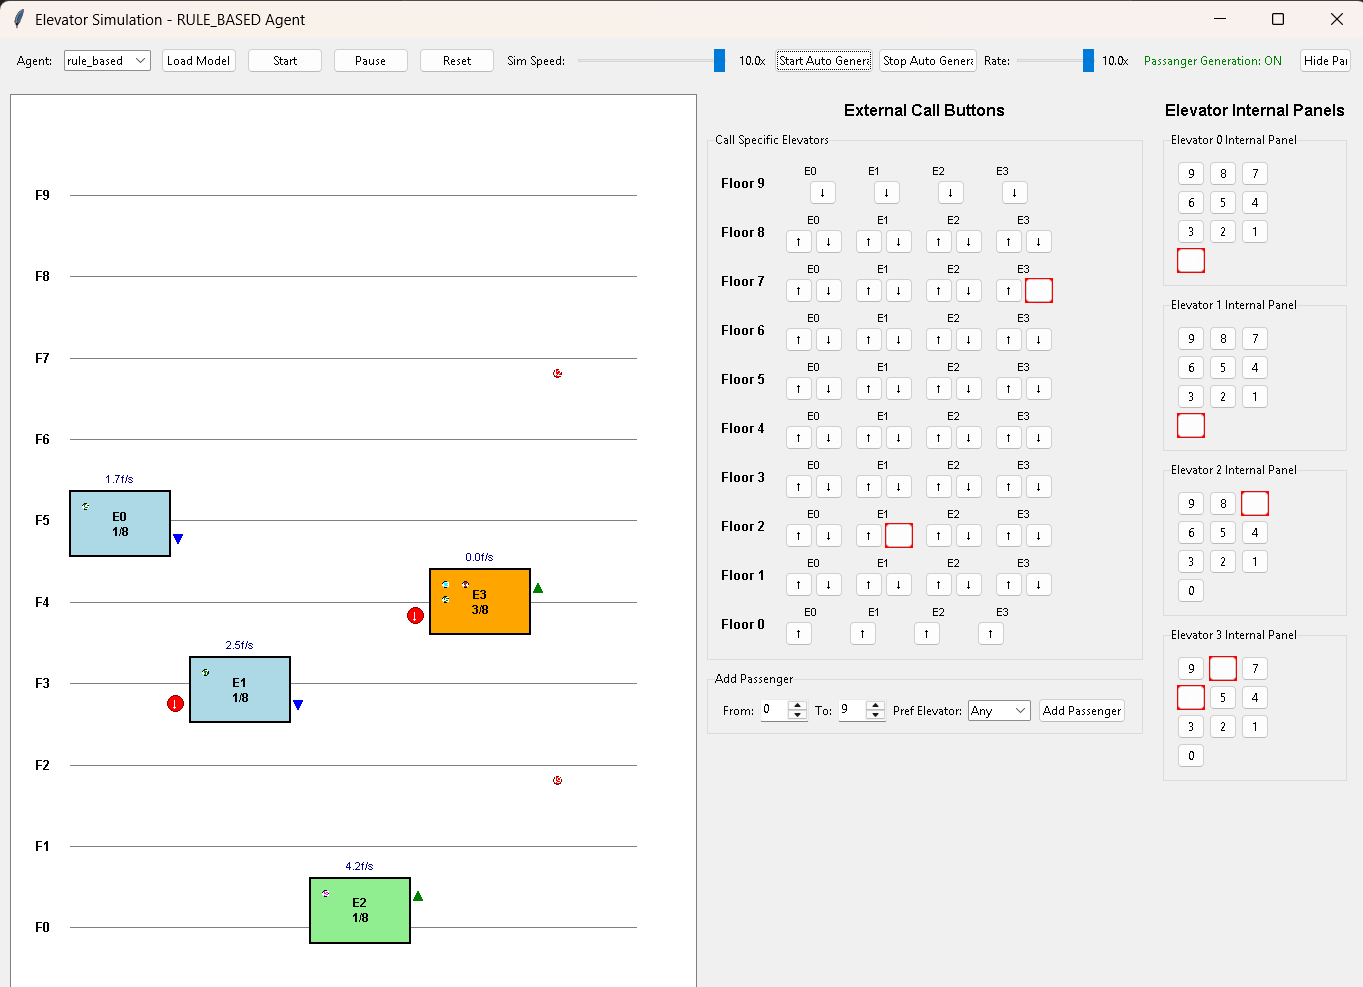
\includegraphics[width=\textwidth]{images/simulation.png}
    \caption{Elevator simulation environment.}
    \label{fig:elevator-simulation}
\end{figure}
\begin{figure}[h!]
    \centering
    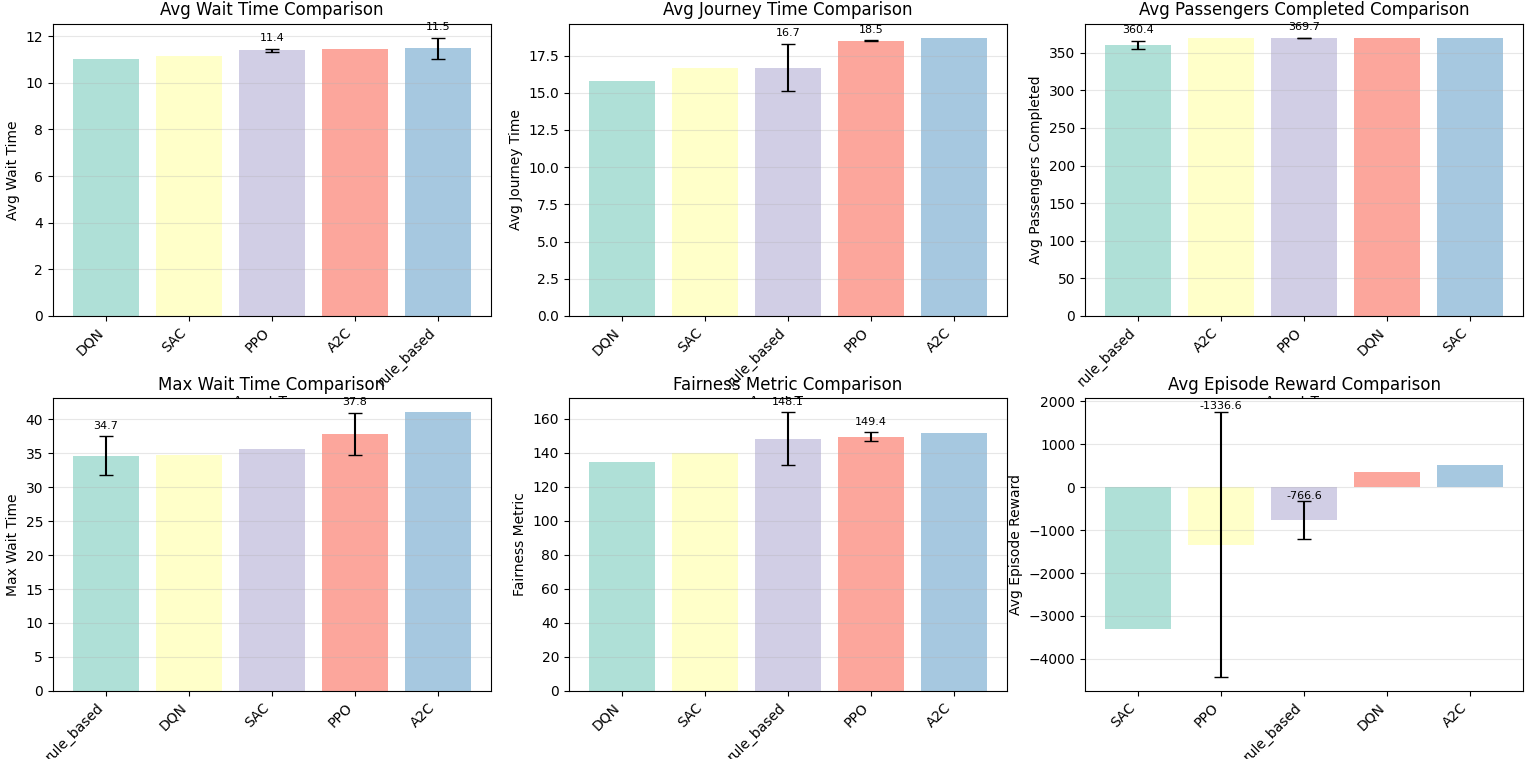
\includegraphics[width=\textwidth]{images/model_comparison.png}
    \caption{Model comparisons:- PPO, A2C, SAC, DQN, Rule-based system.}
    \label{fig:model-comparison}
\end{figure}
\begin{figure}[h!]
    \centering
    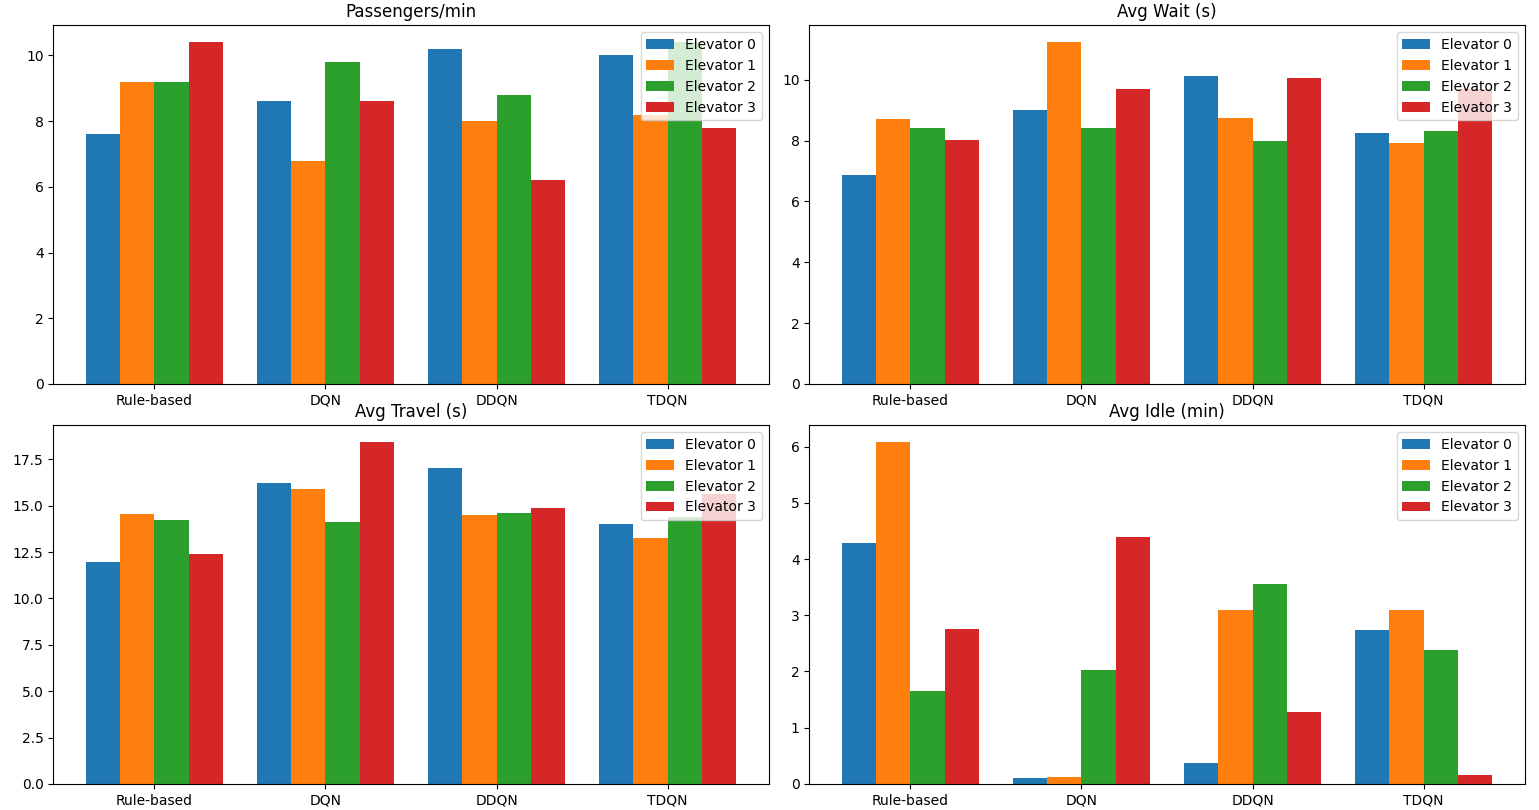
\includegraphics[width=\textwidth]{images/elevator_comparison.png}
    \caption{Comparing elevator performance for DQN, DDQN, TDQN with Rule-based system.}
    \label{fig:elevator-comparison}
\end{figure}
\begin{figure}[h!]
    \centering
    
\includegraphics[width=\textwidth]{images/dqn_training.png}
    \caption{Training progress of DQN vs DDQN vs TDQN over 25 episodes (each of 3600 simulation steps) .}
    \label{fig:dqn-training}
\end{figure}
\begin{figure}[h!]
    \centering
    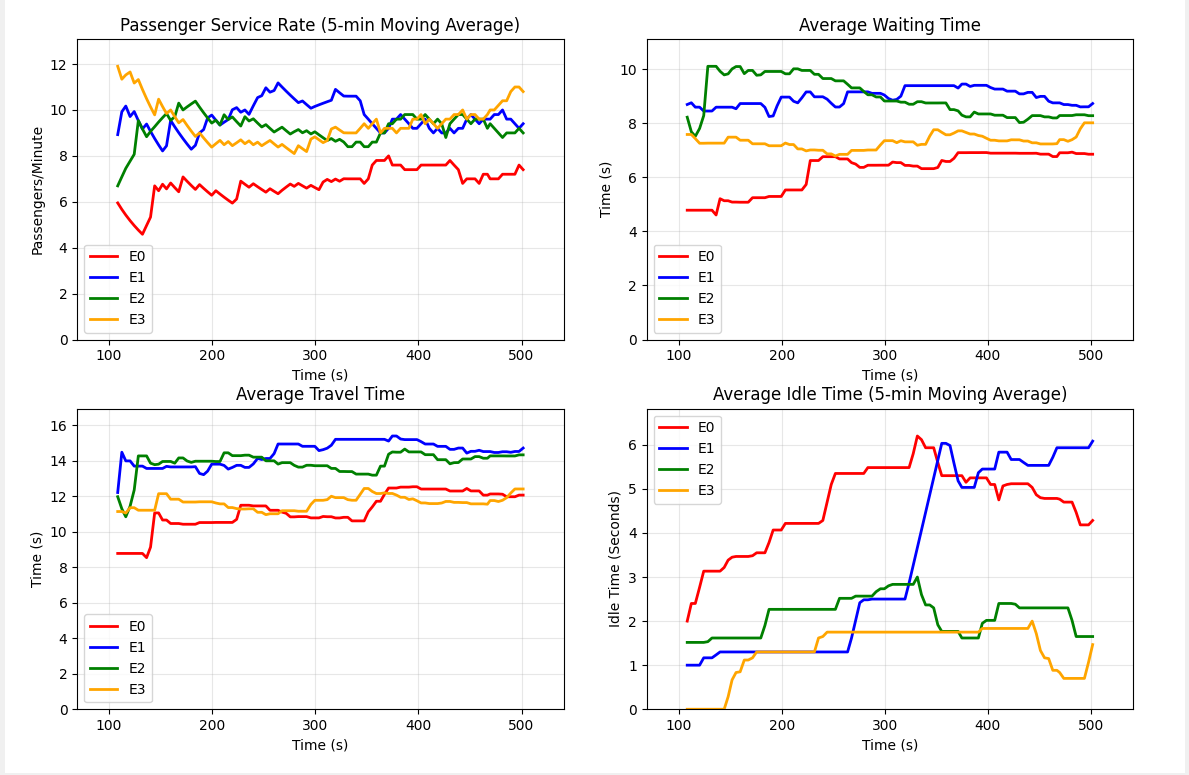
\includegraphics[width=\textwidth]{images/rule_based.png}
    \caption{Performance evaluation of Rule-based system.}
    \label{fig:rule-based-performance}
\end{figure}
\begin{figure}[h!]
    \centering
    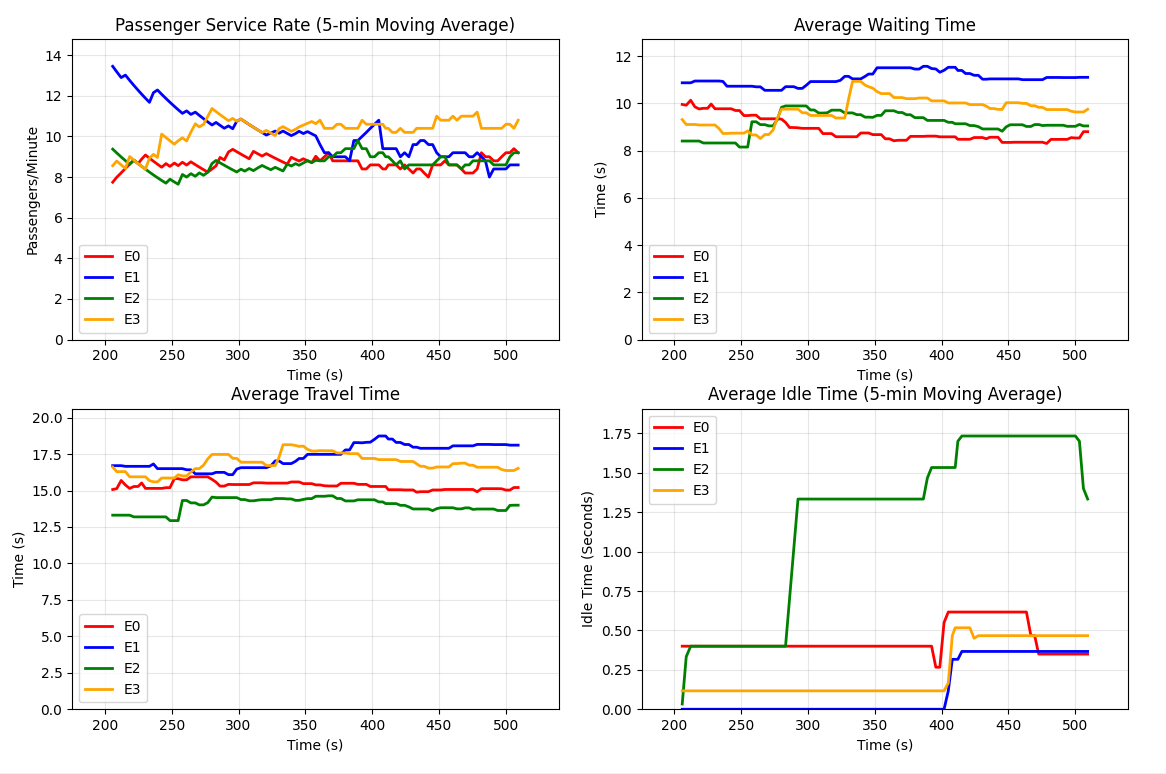
\includegraphics[width=\textwidth]{images/dqn.png}
    \caption{Performance evaluation of DQN.}
    \label{fig:dqn-performance}
\end{figure}
\begin{figure}[h!]
    \centering
    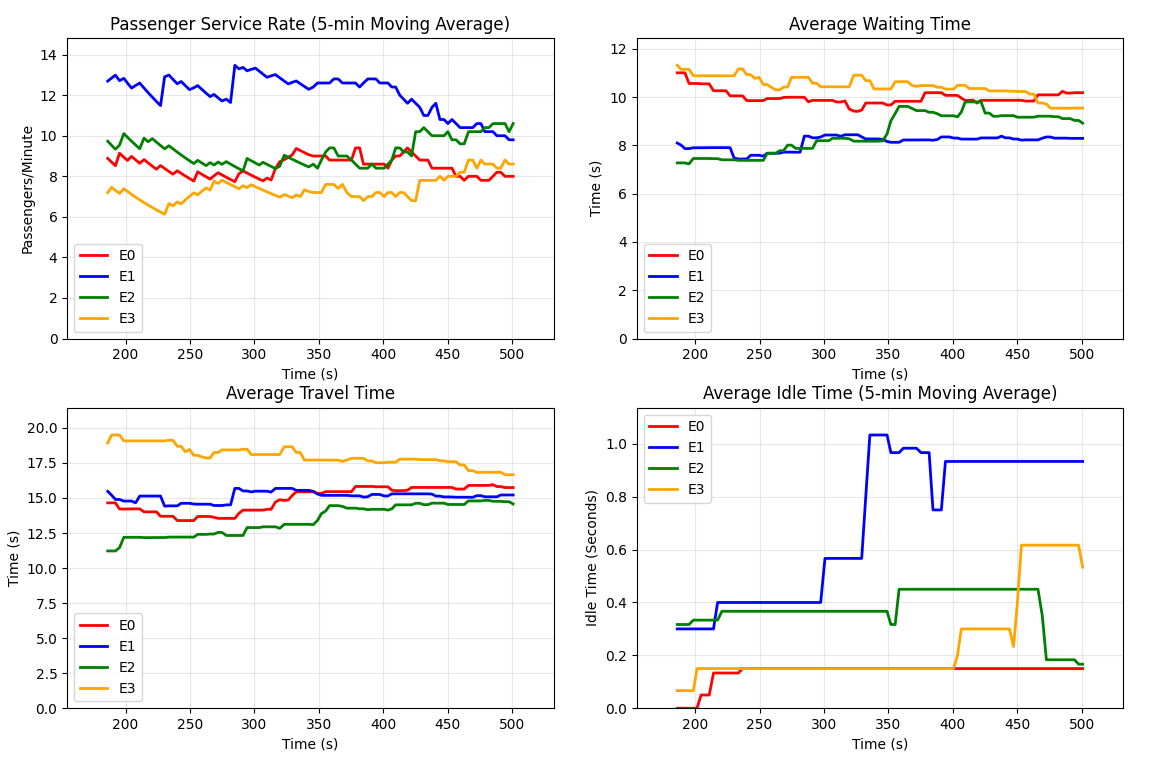
\includegraphics[width=\textwidth]{images/ddqn.png}
    \caption{Performance evaluation of DDQN.}
    \label{fig:ddqn-performance}
\end{figure}
\begin{figure}[h!]
    \centering
    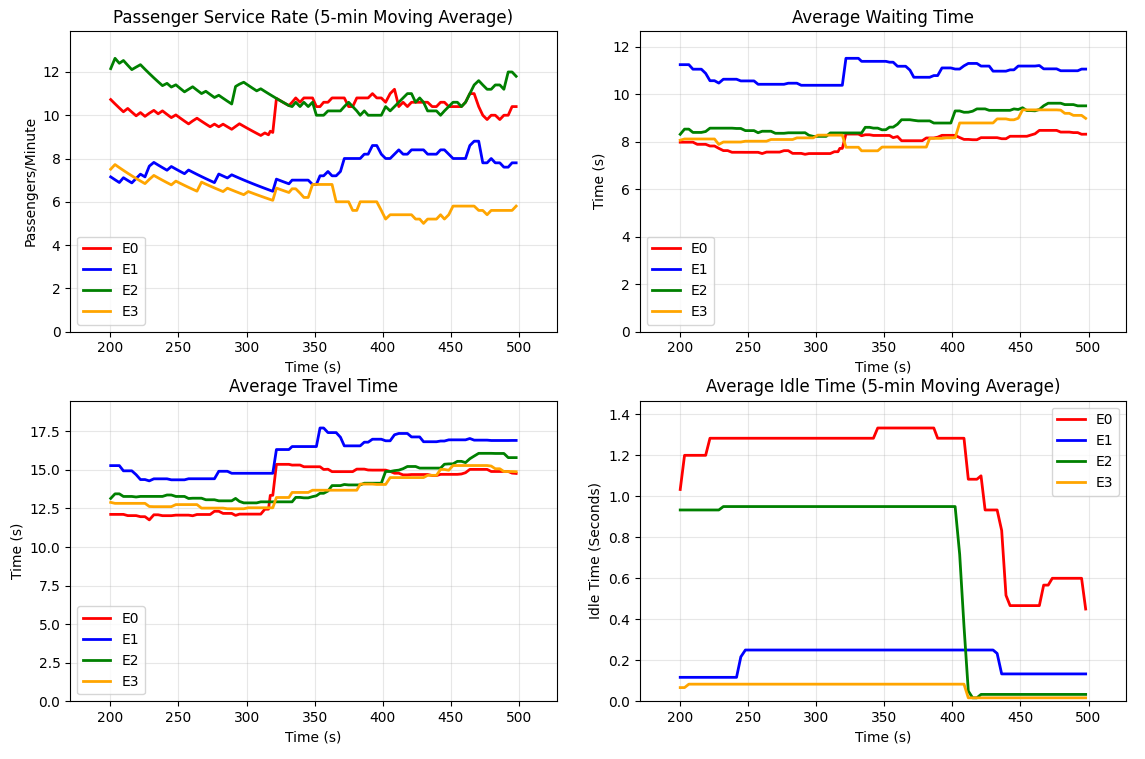
\includegraphics[width=\textwidth]{images/tdqn.png}
    \caption{Performance evaluation of TDQN.}
    \label{fig:tdqn-performance}
\end{figure}

\clearpage                % Force references to start on a clean page
\bibliographystyle{IEEEtran}
\bibliography{report}

\end{document}
